\documentclass{letask}

\begin{document}
\begin{titlepage}
\center % Center everything on the page
 
%----------------------------------------------------------------------------------------
%	HEADING SECTIONS
%----------------------------------------------------------------------------------------

\textsc{\LARGE Московский\\[-0.2cm]Физико-Технический Институт\\[0.1cm]\large (государственный университет)}\\[1.5cm] % Name of your university/college
\textsc{\Large Кафедра общей физики}\\[0.1cm] % Major heading such as course name
\textsc{\large Лабораторная работа \textnumero  4.4.1}\\[0.5cm] % Minor heading such as course title

%----------------------------------------------------------------------------------------
%	TITLE SECTION
%----------------------------------------------------------------------------------------

\HRule
\\[0.4cm]
{ \huge \bfseries Амплитудная\\[0.2cm]
дифракционная решетка}
\\[0.6cm] % Title of your document
\HRule
\\[1.5cm]


 
%----------------------------------------------------------------------------------------
%	AUTHOR SECTION
%----------------------------------------------------------------------------------------

\begin{minipage}{0.4\textwidth}
	\begin{flushleft} \large
		\textsf{Студент}
		
		Ришат \textsc{Исхаков} \\[-0.15cm]
		513 группа
	\end{flushleft}
\end{minipage}
~
\begin{minipage}{0.4\textwidth}
	\begin{flushright} \large
		\textsf{Преподаватель}
		
		Александр Александрович \\[-0.15cm]
		\textsc{Казимиров} % Supervisor's Name
	\end{flushright}
\end{minipage}

\begin{bottompar}
	\begin{center}
		
\includegraphics[width = 80 mm]{logo.jpg}
	\end{center}
	{\large \today}

\end{bottompar}
\vfill % Fill the rest of the page with whitespace

\end{titlepage}

\textbf{Цель работы:} исследовать явления дифракции Френеля и Фраунгофера на щели, изучить влияние дифракции на разрешающую способность оптических инструментов.

\textbf{В работе используются:} оптическая скамья, ртутная лампа, монохроматор, щели с регулируемой шириной, рамка с вертикальной нитью, двойная щель, микроскоп на поперечных салазках с микрометрическим винтом, зрительная труба.

\section{Дифракция Френеля на щели}

Схема установки для наблюдения дифракции Френеля представлена на рис. 1. Световые лучи освещают щель $S_2$ и испытывают на ней дифракцию. Дифракционная картина рассматривается с помощью микроскопа М, сфокусированного на некоторую плоскость наблюдения П.

\begin{figure}[H]
\centering
	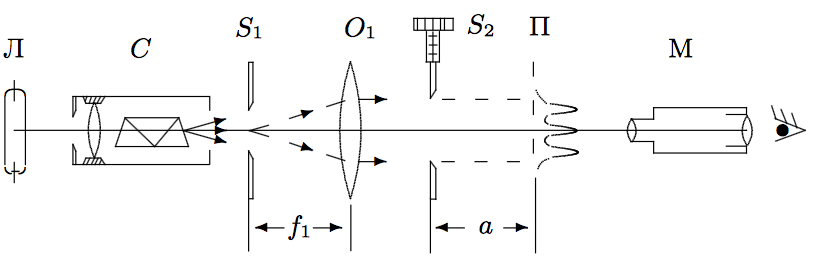
\includegraphics[width = \lw]{img1}
	\caption{Схема установки для наблюдения дифракции Френеля}
	\label{fig:scheme}
\end{figure}


Щель S2 освещается параллельным пучком монохроматического света с помощью коллиматора, образованного объективом $O_1$ и щелью $S_1$, находящейся в его фокусе. На щель $S_1$ сфокусировано изображение спектральной линии, выделенной из спектра ртутной лампы Л при помощи простого монохроматора C, в котором используется призма прямого зрения. 

Распределение интенсивности света в плоскости наблюдения П проще всего рассчитывать с помощью зон Френеля (для щели их иногда называют зонами Шустера). При освещении щели $S_2$ параллельным пучком лучей (плоская волна) зоны Френеля представляют собой полоски, параллельные краям щели. Результирующая амплитуда в точке наблюдения определяется суперпозицией колебаний от тех зон Френеля, которые не перекрыты створками щели. Графическое определение результирующей амплитуды производится с помощью векторной диаграммы — спирали Корню. Суммарная ширина $n$ зон Френеля $\xi_n$ определяется соотношением: 
\[ \xi_n = \sqrt{an\lambda}, \]

где a~--~расстояние от щели до плоскости наблюдения (рис. \ref{fig:scheme}), а $\lambda$~--~длина волны.

\textbf{Измерим значение расстояний при изменении количества темных полос:}

\begin{table}[H]
\centering
\caption{Зависимость расстояния от количества полос}
\begin{tabular}{|c|c|c|c|c|c|}
\hline
$m$          & 5      & 4      & 3      & 2      & 1      \\ \hline
$n$          & 6      & 5      & 4      & 3      & 2      \\ \hline
$\xi_n,~\mkm$          & 0.8    & 1.1    & 1.4    & 1.8    & 2.6    \\ \hline
$2\xi_n,~\mkm $       & 323.8 & 346.6 & 349.7 & 343.4 & 337.0 \\ \hline
$\delta x,~\cm$   & 0.05   & 0.05   & 0.05   & 0.05   & 0.1    \\ \hline
$\epsilon x$ & 0.06   & 0.05   & 0.04   & 0.03   & 0.04   \\ \hline
$\delta \xi,~\mkm$  & 20.2  & 15.7  & 12.4  & 9.5   & 12.9  \\ \hline
\end{tabular}
\end{table}

Построим график зависимости $2 \xi_n (n) $:

\begin{figure}[H]
\centering
  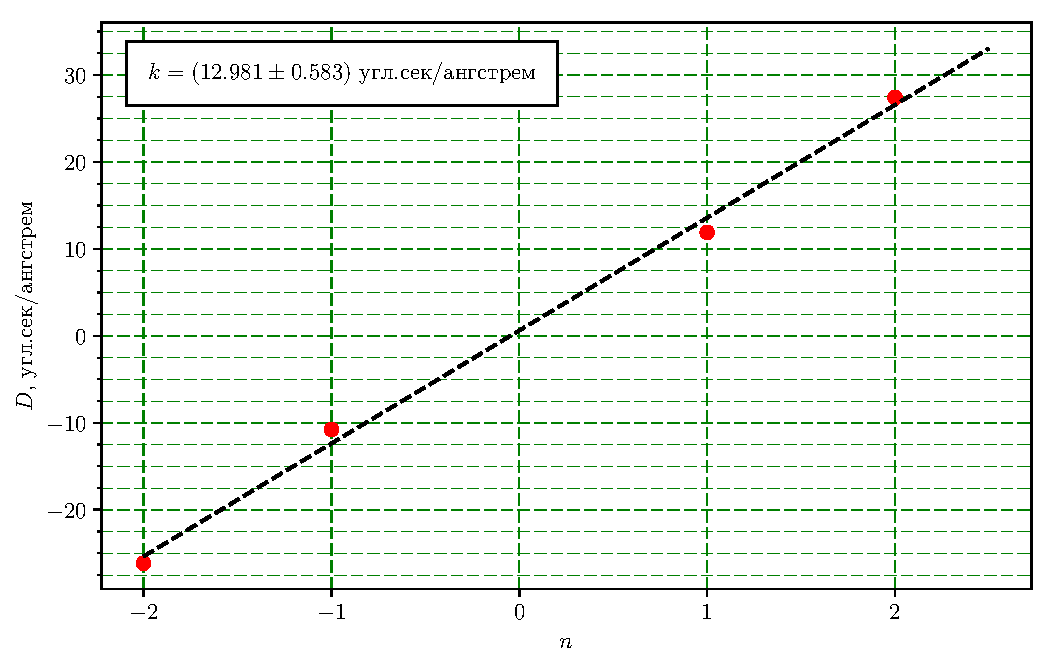
\includegraphics[width = 0.9 \lw]{graph1}
  \caption{График зависимости $2 \xi_n (n)$}
\end{figure}

\section{Дифракция Фраунгофера на щели}

Картина дифракции резко упрощается, когда ширина щели становится значительно меньше ширины первой зоны Френеля. 

Это условие всегда выполняется при достаточно большом расстоянии a от щели до плоскости наблюдения. Дифракционную картину, наблюдаемую в этом случае, принято называть дифракцией Фраунгофера. Исследование такой дифракционной картины заметно облегчается, потому что упрощаются фазовые соотношения.

Дифракцию Френеля и Фраунгофера можно наблюдать на одной и той же установке (рис.~1). Однако при обычных размерах установки дифракция Фраунгофера возникает только при очень узких щелях. Например, при $a \approx 20-40~\cm$ и $\lambda \approx 5 \cdot 10^{-5}~\cm$ получаем $D \ll 0.3~\mm$. Поскольку работать с такими тонкими щелями неудобно, для наблюдения дифракции Фраунгофера к схеме, изображённой на рис. 1 добавляется объектив $O_2$ (рис.~\ref{img:fraung}).

\begin{figure}[H]
\centering
  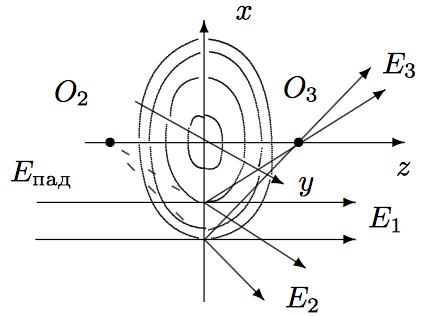
\includegraphics[width = 0.9 \lw]{img2}
  \caption{Схема установки для наблюдения дифракции Фраунгофера на щели}
  \label{img:fraung}
\end{figure}

Дифракционная картина наблюдается здесь в фокальной плоскости объектива $O_2$.

\textbf{Начальные данные:}
\[f_1 = 11~\cm\]
\[f_2 = 12.5~\cm\]

\begin{table}[H]
\centering
\caption{Координаты дифракционных минимумов}
\begin{tabular}{|c|c|c|c|c|c|c|c|c|c|}
\hline
$m$        & -4   & -3   & -2   & -1   & 0   & 1    & 2    & 3   & 4    \\ \hline
$x_m, \mm$ & 0.62 & 0.85 & 1.03 & 1.25 & 1.5 & 1.68 & 1.88 & 2.1 & 2.32 \\ \hline
\end{tabular}
\end{table}

Построим график зависимости $x_m(m)$:

\begin{figure}[H]
  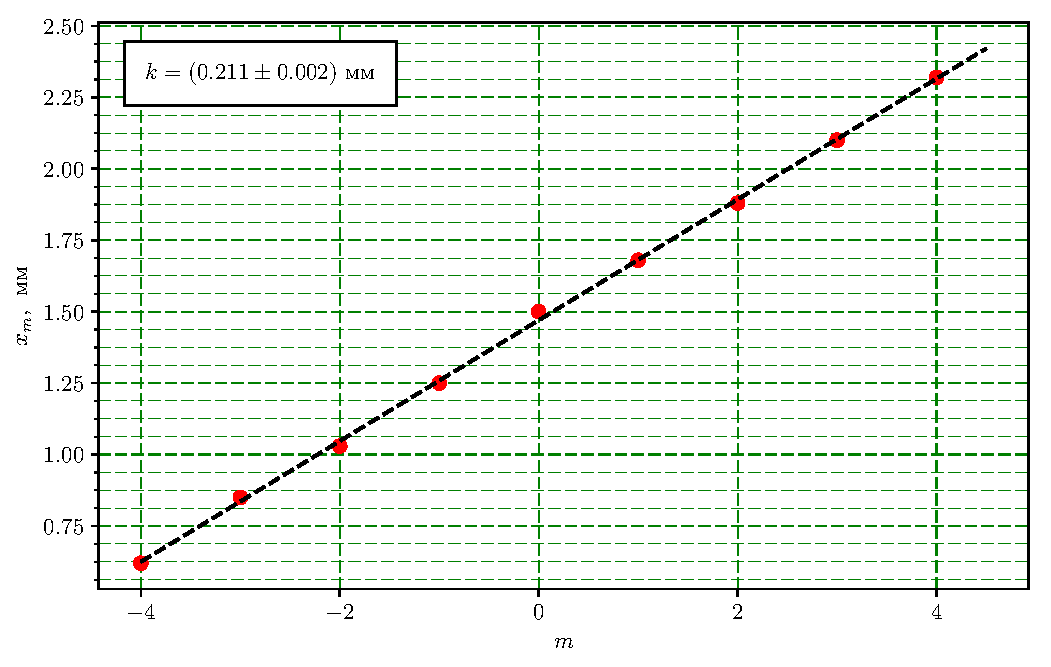
\includegraphics[width = 0.9 \lw]{graph2}
  \caption{Зависимость $x_m(m)$}
\end{figure}

Рассчитаем ширину щели $b$:
\[b = \dfrac{f_2 \lambda}{k} = 0.32~\mm \]

\section{Дифракция Фраунгофера на двух щелях}

\begin{figure}[H]
\centering
  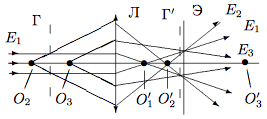
\includegraphics[width = 0.9 \lw]{img3}
  \caption{Схема установки для наблюдения дифракции Фраунгофера на двух щелях}
  \label{img:fraung_2}
\end{figure}


Для наблюдения дифракции Фраунгофера на двух щелях в установке (рис. \ref{img:fraung}) следует заменить щель $S_2$ экраном Э с двумя щелями (рис. \ref{img:fraung_2}). При этом для оценки влияния ширины входной щели на чёткость ди- фракционной картины вместо входной щели $S_1$ следует поставить щель с микрометрическим винтом. Два дифракционных изображения входной щели, одно из которых образовано лучами, прошедшими через левую, а другое — через правую щели, накладываются друг на друга.

Если входная щель достаточно узка, то дифракционная картина в плоскости П (рис. \ref{img:fraung}) подобна той, что получалась при дифракции на одной щели (рис. \ref{img:fraung_2}), однако теперь вся картина испещрена рядом дополнительных узких полос. Наличие этих полос объясняется суперпозицией световых волн, приходящих в плоскость наблюдения через разные щели экрана Э.

 \begin{enumerate}
  \item Определим координаты $x_1, x_2$ самых удаленных друг от друга темных полос внутри первого максимума, а также координату центра максимума:
\[x_1 = 1.38~\mm \] 
\[x_2 = 1.74~\mm \]
Всего в первом максимуме обнаружено $n=5$ светлых полос, поэтому расстояние между ними равно:
\[\delta x = \dfrac{x_2 - x_1}{n} = \dfrac{0.36}{5} = 0.072~\mm \]
Теперь можно найти расстояние между щелями:
\[d = \dfrac{f_2 \lambda}{\delta x} = 0.9~\mm \]
  \item Исследуем влияние пространственной когерентности на видность картины.
  \[b_0 = \dfrac{f_1 \lambda}{d} = 67~\mkm \]
  Экспериментально: 
  \[b_{0 \text{эксп}} = 110~\mkm \]
\end{enumerate}

\section{Влияние дифракции на разрешающую способность оптического инструмента}

Установка, представленная на рис. \ref{img:dif}, позволяет исследовать влияние дифракции на разрешающую способность оптических инструментов.
Как уже было выяснено, линзы $O_1$ и $O_2$ в отсутствие щели $S_2$ создают в плоскости П изображение щели $S_1$, и это изображение рассматривается в микроскоп М. Таким образом, нашу установку можно рассматривать как оптический инструмент, предназначенный для получения изображения предмета. При этом коллиматор (щель $S_1$ и объектив $O_1$) является моделью далёкого предмета, а объектив $O_2$ и микроскоп М составляют зрительную трубу, наведённую на этот предмет.

Если перед объективом $O_2$ зрительной трубы расположить щель $S_2$, то изображение объекта будет искажено дифракцией на щели $S_2$. Чем меньше ширина $D_0$ этой щели, тем сильнее искажение. Качественной характеристикой этих искажений может служить минимальное угловое расстояние $\phi_{min}$ между объектами (источниками), которые ещё воспринимаются как раздельные.

\begin{figure}[H]
\centering
  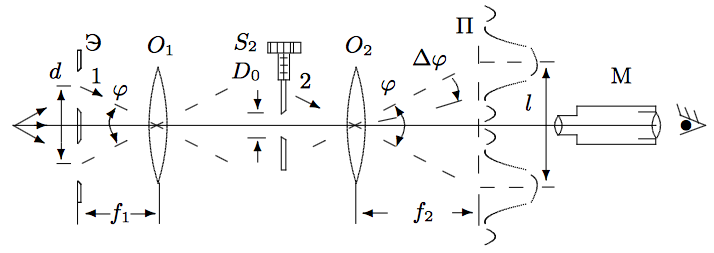
\includegraphics[width = 0.9 \lw]{img4}
  \caption{Схема установки для исследования разрешающей способности оптического инструмента}
  \label{img:dif}
\end{figure}

\begin{enumerate}
  \item При помощи микроскопа измерим расстояние между щелями:
  \[ d = 0.31 - 0.17~\mm = 0.8~\mm \]
  \item Найдем ширину $D_0$ щели $S_2$ при которой пропадают различия между изображениями двух щелей:
  \[ D_0 = \dfrac{f_1 \lambda}{d} = 0.75~\mm \]
  
  \item Теперь подберем экспериментально ширину $D_0$ щели $S_2$ такой, чтобы два изображения видимые в микроскоп были максимально размыты, но при этом еще видимы:
  \[ D_{0 \text{эксп}} = 0.8~\mm \]
\end{enumerate}

\section{Вывод}
Мы исследовали явления дифракции Френеля и Фраунгофера на щели, посчитали ширину щели теоретически и экспериментально.
\end{document}
